\chapter{Choices in Technologies}
\label{ch:techchoices}
In this chapter, we outline the technologies we choose, and the reasoning for choosing them.

\section{Backend}
\label{sec:techbackend}
The backend is divided into two parts, the signing server and the verification service.

The signing service is implemented in the Kotlin programming language~\cite{kotlin} using the Ktor framework~\cite{ktor}.
The verification servie is implemented in the Go programming language~\cite{golang}.

We chose to split the backend into two because signature verification has to be available both online and offline.
The verification service being separate allows us to ship a smaller program,
and since Go binaries are always statically linked we don't have to worry about shipping dependencies.

For the signing service we chose Kotlin because it is a modern and concise programming language,
providing guaranteed null safety, coroutines for asynchronous programming, higher-order functions and more,
and it's genuinely nice to program in.
Kotlin offers seamless Java interopability, allowing us to make use of the excellent and extensive Java ecosystem.

Using two different programming languages and sets of libraries,
implementing common formats and protocols independently from specification alone,
allows us to hedge against the risk of some flaws in the libraries: if a library used in the signing service produced flawed output,
it would likely be discovered by the verification service since it uses a different implementation of the same concepts.
The exact same flaw being present in two different libraries implemented in different programming languages is rather small.

On top of that, we can test ourselves how well we've specified the protocols and formats:
if these two services can be used together without problems, the specification was precise enough.
If not, we learn where we must improve it, which is a win-win situation.

\section{Frontend}
\label{sec:techfrontend}

Given that the frontend must support the three desktop operating systems Microsoft Windows, GNU/Linux as well as Apple MacOS,
the technological choices available to us are limited.
On the desktop, we could use the \gls{JVM} platform and the JavaFX \gls{GUI} library, whereas on the phones
we could use Flutter~\cite{flutterframework}.
However, developing three applications on five platforms using two new-to-us frameworks and programming languages
would take a lot more time and resources than what is available to us in the scope of this thesis.

In order to reduce complexity and enable code reuse, we decide to implement the frontend as a web application.
Web frontents are capable of running in any modern web browser regardless of platform, be it mobile or desktop.
We're not happy about this, as we would much rather use mature, strongly-typed and well-designed languages and frameworks,
but we're forced to make this compromise in order to meet our objectives in the time available.
In order to reduce the pain, we will use TypeScript, which is a typed superset of JavaScript~\cite{loltypes}.

\subsection{Client-Side File Hashing in the Web Browser}
\label{subsec:browserhashing}
However, the decision to implement the frontend as a web application presents us with a challenge:
hashing the files to be signed client-side in the web browser itself.
If we had implemented "proper" client applications this would've been easy, but in a web browser and using its
JavaScript language not so much: it simply wasn't designed with file I/O and CPU-intensive cryptographic functions in mind.

The easiest solution would be to upload the files to be signed to the server and hash them there,
but this would be a clear violation of the least-information principle (the server doesn't need the file, only the hash)
and a breach of user privacy.
Nevermind the fact that signing large files could take a very long time over slow network connections,
and turn out to be quite expensive for mobile users billed for data by volume.

Another solution would be to ask the user to enter the file hashes instead of selecting files,
but this would be very user-unfriendly and most likely too much to ask from many users.

It is clear we must find a way to hash files in the web browser itself.
In order to achieve this we have found the following options:

\begin{enumerate}
    \item Using the browser-implemented \texttt{SubtleCrypto}~\cite{subtlecrypto} \gls{API}
    \item Using the \texttt{CryptoJS}~\cite{cryptojs} JavaScript implementation
    \item Using a \gls{WASM}-based implementation
\end{enumerate}

Each of these options comes with a number of advantages and disadvantages, as discussed in more detail in the following sections.

\subsubsection{Using SubtleCrypto}
\label{subsubsec:subtlecrypto}
The \texttt{SubtleCrypto} class offers the \texttt{digest(algorithm, data)} method~\cite{subtlecrypto}, which can be used to
calculate \gls{SHA-256} checksums.
The advantage of using this implementation is that it is available in all modern browsers\footnote{Where modern browsers means Mozilla Firefox, Google Chrome/Chromium, and Microsoft Edge, not older than the respective versions available in 2018},
and since it's executed with native code, being able to take advantage of \gls{AVX2} instructions, instead of JavaScript it should be quite fast.
There's a major drawback though: hashing a large amount of data progressively is not supported, the data has to be
passed to the function en bloc, as seen in listing~\ref{lst:subtlecrypto}.

\begin{lstlisting}[caption={Using SubtleCrypto for calculating SHA-256 checksums}, captionpos=b, language=JavaScript, label={lst:subtlecrypto}]
    crypto.subtle.digest("SHA-256", data).then(hash => {
    console.log(
    // convert ArrayBuffer to hex string
    Array.from(new Uint8Array(hash)).map(
    b => b.toString(16).padStart(2, '0')
    ).join('')
    );
    });
\end{lstlisting}
Our testing showed that selecting files larger than 200MB crashes Firefox tabs when trying to read their contents
into memory before we could pass it to the \texttt{digest} function.
If we assume the users will only ever select small files this should not pose a problem, but unfortunately it's not safe to assume this.

\subsubsection{Using CryptoJS}
\label{subsubsec:cryptojs}
\texttt{CryptoJS} does not have the limitation of \texttt{SubtleCrypto} and supports progressive hashing\footnote{
By progressive hashing we mean the ability to pass to the hash function the data piece by piece in order to avoid holding all of it in memory at once.},
as seen in listing~\ref{lst:cryptojsprogressive}.

\begin{lstlisting}[caption={Progressive SHA-256 hashing using CryptoJS},captionpos=b,language=JavaScript,label={lst:cryptojsprogressive}]
    const sha256 = CryptoJS.algo.SHA256.create();

    sha256.update("Message Part 1");
    sha256.update("Message Part 2");
    sha256.update("Message Part 3");

    const hash = sha256.finalize();
\end{lstlisting}

The advantage of using \texttt{CryptoJS} over \texttt{SubtleCrypto} is, as mentioned, the ability to hash piece-wise.
The disadvantage is that we need to load a third-party JavaScript library, using built-in functionality would be preferable.
And since JavaScript is an interpreted language, using it to calculate the checksums would result in significantly worse performance.
This is a problem especially on mobile devices limited in compute and memory resources as well as battery capacity.
Since we want to support mobile devices properly, and don't want to limit users to small files, we must do better.

\subsubsection{Using a WASM-based implementation}
\label{subsubsec:wasmhashing}
\gls{WASM} provides a low-level virtual machine in the web browser itself,
running machine-independent binary code, comparable to the \gls{JVM} or the \gls{CLR},
albeit much simpler and much less sophisticated.
By using this virtual machine we should be able to run code at near-native speed written in a statically-typed, compiled language such as Rust, C/C++ or Go.
Thus we expect significant performance gains over a JavaScript-based implementation.
While developing the \gls{WASM}-based hashing programmes, we encountered some interesting challenges, as described in the following paragraphs.

\paragraph{CORS Policy} While JavaScript can be executed simply by pointing the browser at a local \gls{HTML} file, the same doesn't work for \gls{WASM}.
The browser's security policy forbids it due to its \gls{CORS} rule~\cite{cors}.
We solved this by starting the \gls{HTTP} server built in to Go's standard library and having the browser load the \gls{WASM} binary through \gls{HTTP}.
The code is in appendix~\ref{chap:appendix_golangwebserver}.
For the Rust-based implementation we used the built-in web server of webpack~\cite{webpack}.

\paragraph{JavaScript/WASM Compatibility} The Golang project conveniently provides a file containing the necessary boilerplate code to load, start and interact with \gls{WASM} programmes called \texttt{wasm\_exec.js}.
But there's a catch: for each version of Go, the version of the accompanying \texttt{wasm\_exec.js} file used must match precisely.
If it doesn't, the code will crash with a segmentation fault.
It took us quite some time to figure out why the code we'd written only a few days prior would segfault now with no changes made to it.

\paragraph{Passing data} Functions written in Go intended to be used from the JavaScript side of things need to have a very specific signature.
As can be seen in listing~\ref{lst:funcsignaturewasm}, there is no typing: all arguments passed to the function are of type \texttt{js.Value} and the return value must be of type \texttt{interface\{\}}\footnote{This is Go's equivalent of Java's \texttt{Object}, it could be anything.}.
This posed us with the challenge of detecting the types and casting the data passed accordingly.

\begin{lstlisting}[caption={Golang WASM function signature}, captionpos=b, language=Go, label={lst:funcsignaturewasm}]
    func f(this js.Value, arg js.Value) interface{} {}
\end{lstlisting}

We've worked on this for hours, producing ugly reflection-based hacks, until we decided to just agree on the types of the arguments and return values beforehand despite the open function signature.
Now all that's needed is a little boilerplate to convert a JavaScript \texttt{Uint8Array} to a Golang \texttt{[]byte}, as seen in listing~\ref{lst:jscastingtogo}.

\begin{lstlisting}[caption={Uint8Array to {[]}byte}, captionpos=b, language=Go, label={lst:jscastingtogo}, captionpos=b]
    func progressiveHash(this js.Value, in []js.Value) interface{} {
        array := in[0]
        buf := make([]byte, array.Get("length").Int())
        js.CopyBytesToGo(buf, array)
        return this
    }
\end{lstlisting}

\paragraph{Goroutines} Go features its own concurrency primitive called Goroutines.
From a programmers' perspective, they can be used like threads, but they carry much less overhead.
Communication between goroutines is achieved by using so-called channels, which on a high level are comparable to queues.
Unfortunately, the \gls{WASM} specification wasn't drafted with this kind of concurrency in mind.
Go is forced to unwind and restore the call stack when switching between goroutines, which is very expensive~\cite{lolnogoroutines}.
We rewrote the Go programme to work without them, and we've seen a small but significant performance improvement.

\paragraph{Rust based WASM}
As the Go implementation also includes the Go runtime,
which makes the wasm file much larger,
and starts a programme that will run continuously in the background it isn't the optimal choice for creating a WebAssembly implementation.
As neither of us knows any other of the other languages that compile to WebAssembly well, we excluded them at first.
However with the drawbacks of the Go based implementation we decided to try to implement a Rust-based version as well,
in order to see how they compare both in performance and ease of development.


\subsection{Performance Comparison}
\label{subsec:perfcomphashing}
No one likes waiting for slow software to do its work, and neither do we.
This is why we decided to compare the performance of the aforementioned options in a simple test:
we measure the time it takes for the browser to calculate the checksum of 1GB of random data using the aforementioned methods.
The code used for each example is in appendix~\ref{ch:appendix-in-browser-hashing-code}.
The tests were run on Debian 10 using Firefox 69 on an Intel i7-8550U.
The results can be seen in figure~\ref{fig:hashingperformance}.

As expected, the in-browser \texttt{SubtleCrypto}-implementation is the fastest, followed by the Rust-based implementation.
JavaScript is so ridiculously slow it's not even trying to compete.
In order to provide a reference to compare the hashing speeds to we include the performance of the \texttt{openssl} command-line programme.

\begin{figure}
    \begin{center}
        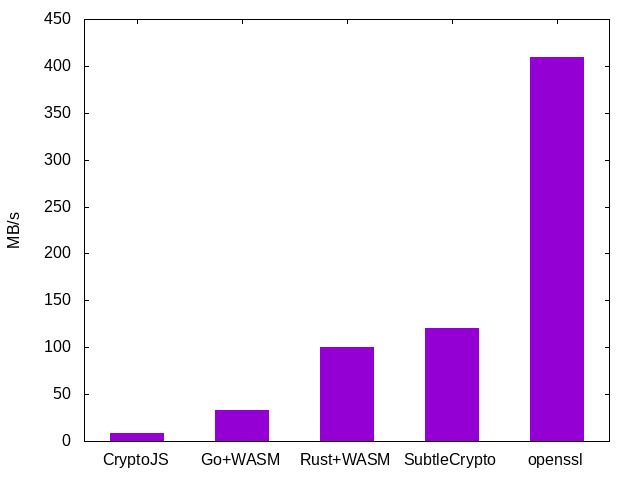
\includegraphics[width=0.7\linewidth]{images/hashingperformance.png}
        \caption{Hashing speed in MB/s (higher is better)}
        \label{fig:hashingperformance}
    \end{center}
\end{figure}


\subsection{Deciding On The In-Browser Hashing Implementation}
\label{subsec:deciding-on-the-in-browser-hashing-implementation}
It is clear from figure~\ref{fig:hashingperformance} that \texttt{SubtleCrypto} is the fastest of the options we tried.
Unfortunately, since it doesn't support piece-wise hashing we're forced to pick the next-fastest option,
the Rust-based implementation running in the \gls{WASM} \gls{VM}.

\section{Evolution of the Signing Protocol}
\label{sec:signingprotocol}

\subsection{Original Protocol}\label{subsec:original-protocol}
The original protocol is based on our work in Projekt 2~\cite{projekt2}.

\subsection{Flaws of the Original Protocol}\label{subsec:flaws-of-the-original-protocol}
The original design employed a server-side secret nonce to generate the nonce used in the \gls{OIDC} authentication request,
which needed to be kept in memory until the signer returned with the ID token from their trip to the \gls{IDP}.
This could be abused to \gls{DoS} the signing server, and it made this part of the signing server stateful.

Furthermore,
for the verification of the signature all documents that were signed together needed to be present at the time of verification,
since their hashes were incorporated in the \gls{OIDC} nonce.

Moreover, multi-signatures, while technically possible, were made impractical for some applications:
If a single person wishes to sign multiple documents at once that will be used together,
(for example, an apartment rental contract, house rules, and a bank deposit confirmation)
this won't be a problem.
However, if multiple, independent documents are to be signed together
(for example, a company sending 50 bills to 50 different customers),
having to send each customer all the bills is just silly.

\subsection{Draft 1: Making the Protocol stateless}\label{subsec:draft-1:-making-the-protocol-stateless}
Since storing the secret nonce on the signing server is undesirable,
we thought about changing the protocol to make this part stateless.

To achieve this, we introduce two more nonce-like values called \texttt{seed} and \texttt{salt}.
The \texttt{seed} is a randomly generated value that is used to verify the id token when the signer returns from the \gls{IDP}.
The \texttt{salt} is the \gls{MAC} of the document hash(es) concatenated with the \texttt{seed}, using a static server side secret as key.

The \texttt{salt} takes the role of the original nonce that was used to construct the \gls{OIDC} nonce and protects against the \gls{IDP} gaining knowledge of the signed hashes and to protect against the \gls{IDP} learning about the document hashes.

The signing server returns both the \texttt{seed} and the \texttt{salt} to the client,
which then constructs the \gls{OIDC} nonce.
The \gls{OIDC} nonce is now the \gls{MAC} of the list of hashes with the \texttt{salt} used as key.

When the signer returns to the signing server, it presents the \texttt{seed}, \texttt{salt}, the hashes and ID token.
Using the \texttt{seed} and the static secret the server can reconstruct the \texttt{salt} and verify that the presented \texttt{salt} is the same.

This functions as a \gls{CSRF} protection of a malicious \gls{IDP} requesting signatures using past values,
while also allowing us to keep the signing server stateless.

After this step the \texttt{seed} will not be used anymore and therefore doesn't need to be in the signature document.
The \gls{OIDC} token will then be verified with the \texttt{salt} and the hashes.

\subsection{Draft 2: Improving signing of multiple documents}\label{subsec:draft-2:-improving-signing-of-multiple-documents}
Even with the improvements in draft 1 (section~\ref{subsec:draft-1:-making-the-protocol-stateless}),
only one signature file will be generated for multiple documents, incorporating all document hashes irrevocably linked together.
Verifying the signature would require having all documents present, which is impractical.

To solve this, our first idea was to include the hashes of the other documents, signed together,
and then generate a signature for each file.
The sorted list of hashes is fed to the \gls{MAC} function in the verification step.
This however would leak information about the other documents, as they would be just plain hashes.
We put a lot of thought into minimising the amount of information all involved actors learn,
such as masking the document hash from the \gls{IDP}, and we're not satisfied with a solution where the other recipients learn
about unrelated document hashes just because they were signed together.

The better solution for this would be to generate a \gls{MAC} of each hash with the \texttt{salt} as key and include that in the signature file,
with the \gls{OIDC} nonce just being the hash of the sorted \gls{MAC}s.

This way the verifiers' own \gls{MAC} can be generated during verification with the other \gls{MAC}s just being used as additional input parameters without leaking the hashes of the documents.
Assuming the \gls{HMAC} function used is secure,
the only information that the receiver of the signature file could learn is the number of the documents that were signed together.

\section{Signature Format}
\label{sec:signatureformat}

\subsection{Original Format}
Our original choice for the signature format is based on our work in Projekt2 which contained the following fields:

\begin{itemize}
    \item signature (Base64)
    \item signature format (\gls{RSA-PSS}, \gls{Ed25519}, ?)
    \item signature hash algorithm (\gls{SHA}256, \gls{SHA}3, ?)
    \item timestamp according to \gls{RFC} 3161\footnote{\url{https://tools.ietf.org/html/rfc3161}}
    \item public key (\gls{PEM})
    \item issuing \gls{CA} (\gls{PEM})
    \item subject
    \item validity
    \item level
\end{itemize}

This format would be encoded as a protobuf message in order to not have an overly verbose file(as opposed to xml), but still having a schema and deterministic encoding(as opposed to json).

\subsection{Adding LTV}
During our work on this thesis we wanted to add \gls{LTV}, which meant adding all the certificate chains, \gls{OCSP} responses and \gls{CLR} of all involved parties, as well as a possibility to refresh the timestamps (yearly).
While experimenting with parsing and generating the timestamp data and understanding the format we noticed, that we were reinventing the wheel a bit in our format. A lot of the info we wanted to include was already present by using a standard \gls{PKCS}\#7 signature with enveloped data.
This means we just need to specify how this enveloped data looks like and how we wrap all the timestamps with the \gls{LTV} information in the protobuf message.

\subsection{Final Format}

First the specification of the enveloped data in the \gls{PKCS}\#7 signature

\begin{itemize}
    \item Hash of the document
    \item used hashing algorithm
    \item key for the \gls{MAC}
    \item \gls{MAC} used
    \item list of the \gls{MAC}s of all other documents that were signed together (needed for link between ID token and signature)
    \item signature level (advanced/qualified)
    \item ID token
    \item \gls{CA} chain of the \gls{IDP}
    \item \gls{OCSP} response for the \gls{IDP} \gls{CA}
    \item \gls{CRL} for the \gls{IDP} \gls{CA}
\end{itemize}

The \gls{PKCS}\#7 encoded signature together with the \gls{OCSP} response and \gls{CRL} of the signing \gls{CA} will be the message that is hashed in the message imprint of the \gls{RFC}3161 timestamp.

To refresh the signature the included timestamp and the \gls{OCSP} response and \gls{CRL} of the timestamping \gls{CA} will be used as the message that is hashed in the message imprint of the next \gls{RFC}3161 timestamp.
